%%%%%%%%%%%%%%%%%%%%%%%%%%%%%%%%%%%%%%%%%
% Academic Title Page
% LaTeX Template
% Version 2.0 (17/7/17)
%
% This template was downloaded from:
% http://www.LaTeXTemplates.com
%
% Original author:
% WikiBooks (LaTeX - Title Creation) with modifications by:
% Vel (vel@latextemplates.com)
%
% License:
% CC BY-NC-SA 3.0 (http://creativecommons.org/licenses/by-nc-sa/3.0/)
%
% Instructions for using this template:
% This title page is capable of being compiled as is. This is not useful for
% including it in another document. To do this, you have two options:
%
% 1) Copy/paste everything between \begin{document} and \end{document}
% starting at \begin{titlepage} and paste this into another LaTeX file where you
% want your title page.
% OR
% 2) Remove everything outside the \begin{titlepage} and \end{titlepage}, rename
% this file and move it to the same directory as the LaTeX file you wish to add it to.
% Then add \input{./<new filename>.tex} to your LaTeX file where you want your
% title page.
%
%%%%%%%%%%%%%%%%%%%%%%%%%%%%%%%%%%%%%%%%%

%----------------------------------------------------------------------------------------
%	PACKAGES AND OTHER DOCUMENT CONFIGURATIONS
%----------------------------------------------------------------------------------------

\documentclass[11pt]{article}

\usepackage[utf8]{inputenc} % Required for inputting international characters
\usepackage[T1]{fontenc} % Output font encoding for international characters

\usepackage{mathpazo} % Palatino font

\usepackage{graphicx}

\usepackage{minted}

\begin{document}

%----------------------------------------------------------------------------------------
%	TITLE PAGE
%----------------------------------------------------------------------------------------

\begin{titlepage} % Suppresses displaying the page number on the title page and the subsequent page counts as page 1
  \newcommand{\HRule}{\rule{\linewidth}{0.5mm}} % Defines a new command for horizontal lines, change thickness here

  \center{} % Centre everything on the page

  %------------------------------------------------
  %	Headings
  %------------------------------------------------

  % Main heading such as the name of your university/college
  \textsc{\LARGE Swinburne University of Technology}\\[1.5cm]

  % Major heading such as course name
  \textsc{
    \Large
    Bachelor of Engineering\\
    (Software Engineering)\\
    (Honours)
  }\\[0.5cm]

  % Minor heading such as course title
  \textsc{\large ICT40010 Research Report A}\\[0.5cm]

  %------------------------------------------------
  %	Title
  %------------------------------------------------

  \HRule{}\\[0.4cm]

  % Title of your document
  {\huge\bfseries Modern Rendering Pipelines}\\[0.2cm]

  \HRule{}\\[1.5cm]

  %------------------------------------------------
  %	Author(s)
  %------------------------------------------------

  \begin{minipage}{0.4\textwidth}
    \begin{flushleft}
      \large
      \textit{Author}\\
      D.J. \textsc{Holland} % Your name
    \end{flushleft}
  \end{minipage}
  {~}
  \begin{minipage}{0.4\textwidth}
    \begin{flushright}
      \large
      \textit{Supervisor}\\
      Dr.\ Clinton \textsc{Woodward} % Supervisor's name
    \end{flushright}
  \end{minipage}

  % If you don't want a supervisor, uncomment the two lines below and comment the code above
  %{\large\textit{Author}}\\
  %John \textsc{Smith} % Your name

  %------------------------------------------------
  %	Date
  %------------------------------------------------

  \vfill\vfill\vfill % Position the date 3/4 down the remaining page

  {\large\today} % Date, change the \today to a set date if you want to be precise

  %------------------------------------------------
  %	Logo
  %------------------------------------------------

  %\vfill\vfill
  %\includegraphics[width=0.2\textwidth]{placeholder.jpg}\\[1cm] % Include a department/university logo - this will require the graphicx package

  %----------------------------------------------------------------------------------------

  \vfill % Push the date up 1/4 of the remaining page

\end{titlepage}

%----------------------------------------------------------------------------------------

\begin{abstract}
  Hello, and welcome to the abstract page. Nice, right?
\end{abstract}
\pagenumbering{gobble}
\newpage

\tableofcontents
\pagenumbering{gobble}
\newpage
\pagenumbering{arabic}

Great, this seems to work now.

\section{Introduction}
\subsection{yeet}
Hello, I'm the introduction!

\section{wow}
\subsection{this is great}
\subsubsection{whew}
\paragraph{NO NONO}
lorem ipsum dolor sit amet, consectetur adip
lorem ipsum dolor sit amet, consectetur adip
lorem ipsum dolor sit amet, consectetur adip
lorem ipsum dolor sit amet, consectetur adip
lorem ipsum dolor sit amet, consectetur adip
lorem ipsum dolor sit amet, consectetur adip
lorem ipsum dolor sit amet, consectetur adip
\subparagraph{neato:}
lorem ipsum dolor sit amet, consectetur adip
lorem ipsum dolor sit amet, consectetur adip
lorem ipsum dolor sit amet, consectetur adip
lorem ipsum dolor sit amet, consectetur adip
lorem ipsum dolor sit amet, consectetur adip
lorem ipsum dolor sit amet, consectetur adip
lorem ipsum dolor sit amet, consectetur adip
\subsection{this is great}
\subsection{this is great}
\subsection{this is great}
lorem ipsum dolor sit amet, consectetur adip lorem ipsum dolor sit amet, consectetur adip lorem ipsum dolor sit amet, consectetur adip lorem ipsum dolor sit amet, consectetur adip lorem ipsum dolor sit amet, consectetur adip lorem ipsum dolor sit amet, consectetur adip lorem ipsum dolor sit amet, consectetur adip lorem ipsum dolor sit amet, consectetur adip lorem ipsum dolor sit amet, consectetur adip lorem ipsum dolor sit amet, consectetur adip lorem ipsum dolor sit amet, consectetur adip lorem ipsum dolor sit amet, consectetur adip lorem ipsum dolor sit amet, consectetur adip lorem ipsum dolor sit amet, consectetur adip lorem ipsum dolor sit amet, consectetur adip lorem ipsum dolor sit amet, consectetur adip lorem ipsum dolor sit amet, consectetur adip lorem ipsum dolor sit amet, consectetur adip lorem ipsum dolor sit amet, consectetur adip lorem ipsum dolor sit amet, consectetur adip lorem ipsum dolor sit amet, consectetur adip lorem ipsum dolor sit amet, consectetur adip lorem ipsum dolor sit amet, consectetur adip lorem ipsum dolor sit amet, consectetur adip lorem ipsum dolor sit amet, consectetur adip lorem ipsum dolor sit amet, consectetur adip lorem ipsum dolor sit amet, consectetur adip lorem ipsum dolor sit amet, consectetur adip lorem ipsum dolor sit amet, consectetur adip lorem ipsum dolor sit amet, consectetur adip lorem ipsum dolor sit amet, consectetur adip lorem ipsum dolor sit amet, consectetur adip lorem ipsum dolor sit amet, consectetur adip lorem ipsum dolor sit amet, consectetur adip lorem ipsum dolor sit amet, consectetur adip lorem ipsum dolor sit amet, consectetur adip lorem ipsum dolor sit amet, consectetur adip lorem ipsum dolor sit amet, consectetur adip lorem ipsum dolor sit amet, consectetur adip lorem ipsum dolor sit amet, consectetur adip lorem ipsum dolor sit amet, consectetur adip lorem ipsum dolor sit amet, consectetur adip lorem ipsum dolor sit amet, consectetur adip lorem ipsum dolor sit amet, consectetur adip lorem ipsum dolor sit amet, consectetur adip lorem ipsum dolor sit amet, consectetur adip.
\subsection{this is great}
\subsection{this is great}
\subsection{this is great}
vert good sir!

doing some cheeky code blocks\ldots

\usemintedstyle{manni}
\begin{minted}{c}
int main() {
  printf("hello, world");
  return 0;
}
\end{minted}

\begin{minted}{rust}
fn main() {
  let mut app = App::new("Glamour Sandbox", 512, 490);
  let sandbox_layer = SandboxLayer::new("SandboxLayer");
  app.push_layer(Box::new(sandbox_layer));
  app.run();
}
\end{minted}

\begin{figure}\centering
  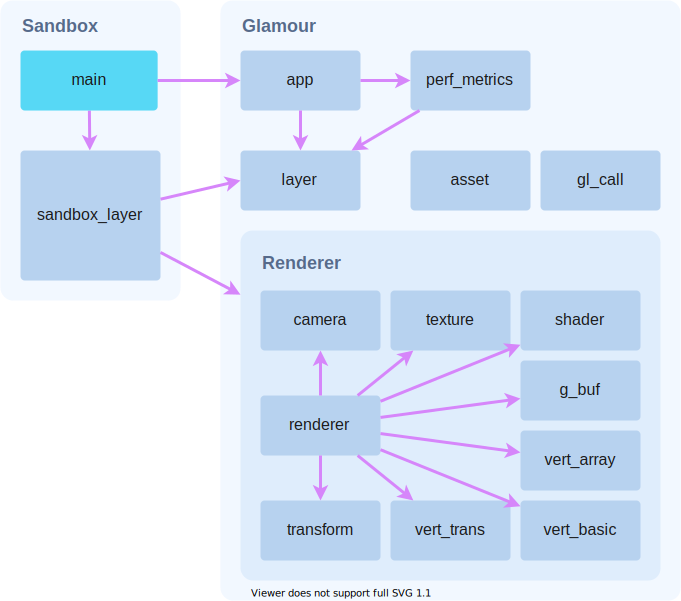
\includegraphics[width=1\columnwidth]{module-graph.png}
  \caption[Short title]{Long title}\label{fig:ff}
\end{figure}

\end{document}
